\documentclass{beamer}

% importations de packages utiles
\usepackage[utf8]{inputenc}  % pouvoir écrire avec des accents
\usepackage[french]{babel}  % francophopnie
\usepackage{hyperref}  % liens clicables dans pdf final
\usepackage{tikz}  % pouvoir tracer des dessins sympas
\usetheme{Boadilla}  % thème de beamer
\usepackage{listingsutf8}  % rendu de "code" (avec config ci-dessous)
\definecolor{lstcolor}{rgb}{0.9,0.95,0.95}
\definecolor{lstcommentcolor}{rgb}{0.,0.2,0.}
\lstset{
  frameround=tttt,
  %autogobble,
  frame=single,
  backgroundcolor=\color{lstcolor},
  % extendedchars=true,
  % basicstyle=\ttfamily\small,
  keywordstyle=\bfseries\color{blue},
  identifierstyle=\bfseries\color{red},
  stringstyle=\bfseries\color{orange},
  commentstyle=\color{lstcommentcolor},
  language=Python,
  keepspaces=True,
  basicstyle=\fontfamily{pcr}\selectfont\small, % monospace it for copypasting
  upquote=true,
  columns=flexible,
  showstringspaces=False,
  literate={é}{{\'e}}1
}
\title{La Concurrence}
\subtitle{Concepts de Langages de Programmation}
\author{Juan-Carlos Barros et Daniel Kessler}
% et c'est parti
\begin{document}
\begin{frame}
  \titlepage
\end{frame}

\begin{frame}
  \tableofcontents
\end{frame}

\section{Introduction}
\begin{frame}
  \frametitle{Introduction: la concurrence en-dehors de l'informatique}
  \begin{itemize}
  \item le cerveau
  \item les rails
  \item \ldots
  \end{itemize}
\end{frame}

\section{Les fondamentaux de la concurrence}
\begin{frame}
  \frametitle{Fondamentaux de la concurrence en informatique}
  \begin{itemize}
  \item Situations en informatique où la concurrence est inévitable
  \item Threads vs Processus
  \item Synchrone vs Asynchrone
  \item Problèmes classiques
  \item Solutions classiques
  \end{itemize}
\end{frame}
\begin{frame}
  \frametitle{Situations en informatique où la concurrence est inévitable}
  \begin{itemize}
  \item Le Système d'Exploitation
  \item Toute application distribuée (par exemple un service web)
  \end{itemize}
\end{frame}
\begin{frame}
  \frametitle{Threads vs Processus}
  \begin{itemize}
  \item Processus: idéal pour déléguer des calculs intensifs
  \item Threads: idéal pour déléguer des opérations I/O
  \end{itemize}
\end{frame}
\begin{frame}
  \frametitle{Communication synchrone vs asynchrone}
  \begin{itemize}
  \item synchrone: \ldots
  \item asynchrone: \ldots
  \end{itemize}
\end{frame}
\begin{frame}
  \frametitle{Problèmes classiques}
  \begin{itemize}
  \item ``race condition''
  \item famine (starvation)
  \item interblocage (deadlock)
  \item $\rightarrow$ sections critiques
  \end{itemize}
  $\rightarrow$ ``jeu de Dekker'' pour illustrer 
\end{frame}
\begin{frame}
  \frametitle{Solutions classiques}
  \begin{itemize}
  \item Verrous
  \item Sémaphores de Dijkstra
  \item Moniteurs
  \item Futures/Promises
  \end{itemize}
\end{frame}
\begin{frame}
  \frametitle{Solutions classiques}
  Le langage de modélisation graphique \textbf{UML} se prête bien à décrire ce
  genre d'outil.
  \par
  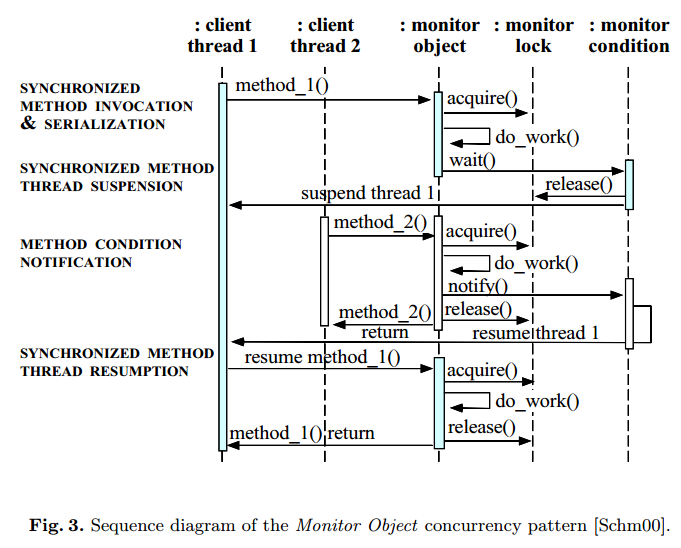
\includegraphics[width=.7\textwidth]{monitor.png}
\end{frame}
\begin{frame}
  \frametitle{Exemple d'implémentation}
  (code Python ou Java)
\end{frame}

\section{Autres paradigmes concurrents}
\begin{frame}
  \frametitle{Autres paradigmes concurrents}
  \begin{itemize}
  \item Transactions
  \item Acteurs
  \item Événements
  \item Coroutines
  \end{itemize}
\end{frame}
\begin{frame}
  \frametitle{Transactions}
  \begin{itemize}
  \item Rendre ``atomique'' la section critique
  \item Idée inspirée des Bases de Donnée
  \item Idée très bien exploitée dans le langage \textbf{Clojure}
    \begin{center}
      [bout de code Clojure]
    \end{center}
  \end{itemize}
\end{frame}
\begin{frame}
  \frametitle{Éviter la mémoire partagée?}
  \begin{itemize}
  \item La mémoire partagée est la source de la plupart des problèmes
  \item Les communications ne devraient se faire que par des \textbf{immuables}
  \end{itemize}
\end{frame}
\begin{frame}
  \frametitle{Modèle d'Acteurs de Hewitt}
  Un \textbf{acteur} peut:
  \begin{itemize}
  \item Envoyer des \textbf{messages} à d'autres acteurs
  \item Créer d'autres acteurs
  \item Décider de son comportement à la prochaine réception de message
  \end{itemize}
  $\rightarrow$ le langage \textbf{Erlang} exploite bien ce modèle
  \begin{center}
    [bout de code Erlang]
  \end{center}
  Plus récemment, le langage \textbf{Scala} s'y prête aussi
  \begin{center}
    [micro-bout de code Scala?]
  \end{center}
\end{frame}
\begin{frame}
  \frametitle{Modèle d'Acteurs de Hewitt}  
  $\rightarrow$ ce modèle se prête bien à une analyse formelle ($\pi$-calculus,
  réseaux de Petri, \ldots)
  \par
  \begin{center}
        [image de réseau de Petri / bout de $\pi$-calculus]    
  \end{center}
\end{frame}
\begin{frame}
  \frametitle{Événements}
  [section peut-être à supprimer]\medskip
  
  Événement: ``message'' d'origine interne ou externe, en attente d'être géré.
  \begin{itemize}
  \item ``event loop''
  \item ``event handlers'' (callbacks)
  \end{itemize}
  $\rightarrow$ utile pour programmer des GUI, mais code difficile à analyser et maintenir
\end{frame}
\begin{frame}
  \frametitle{Coroutines}
  Pas besoin de threads ou process dans les modèles Acteur ou Event-driven, mais ils sont possibles.
  \par\medskip
  Alternative, les coroutines: des routines concurrentes dans le même thread
  \par\smallskip
  $\rightarrow$ exploitées à fond dans le langage \textbf{Go} (``goroutines'')
  \begin{center}
    [bout de code Go]
  \end{center}
\end{frame}

\section{Conclusion}
\begin{frame}
  \frametitle{Conclusion: au-delà de la concurrence}
  Réseaux de neurone!
\end{frame}


\end{document}